\documentclass[10pt,a4paper]{article}

\usepackage[T1]{fontenc}
\usepackage[utf8]{inputenc}
\usepackage[margin=2.5cm]{geometry}
\usepackage{lmodern}
\usepackage{amsmath,amssymb,mathtools}
\usepackage{graphicx}
\usepackage{booktabs}
\usepackage{microtype}
\usepackage{setspace}
\usepackage{parskip}
\usepackage{caption}
\usepackage{placeins}
\usepackage{fancyhdr}
\usepackage{titlesec}
\usepackage{titling}
\usepackage[authoryear]{natbib}
\usepackage{hyperref}
\usepackage{bookmark}

\hypersetup{
  colorlinks=true,
  linkcolor=black,
  citecolor=black,
  urlcolor=black,
  pdftitle={Walk Forward Trend Following and BTC Dominance Mean Reversion in Cryptocurrency Markets},
  pdfauthor={Peter Prendergast}
}
\captionsetup[figure]{position=bottom}
\captionsetup[table]{position=bottom}

\setstretch{1.12}
\setlength{\parskip}{0.30em}
\setlength{\parindent}{0pt}
\setlength{\droptitle}{-1.5cm}
\setlength{\textfloatsep}{9pt plus 2pt minus 2pt}
\setlength{\intextsep}{7pt plus 2pt minus 2pt}
\setlength{\abovecaptionskip}{4pt}
\setlength{\belowcaptionskip}{2pt}
\setlength{\abovedisplayskip}{7pt plus 2pt minus 2pt}
\setlength{\belowdisplayskip}{7pt plus 2pt minus 2pt}

\pretitle{\begin{center}\LARGE\bfseries}
\posttitle{\par\vspace{0.4em}\rule{0.8\textwidth}{0.5pt}\end{center}\vspace{0.8em}}
\preauthor{\begin{center}\normalsize}
\postauthor{\par\end{center}\vspace{-0.6em}}
\predate{\begin{center}\normalsize}
\postdate{\par\end{center}\vspace{0.8em}}

\titleformat{\section}
  {\large\bfseries}
  {\thesection}{0.75em}{}
\titleformat{\subsection}
  {\normalsize\bfseries}
  {\thesubsection}{0.75em}{}
\titleformat{\subsubsection}
  {\normalsize\itshape}
  {\thesubsubsection}{0.75em}{}

\titlespacing*{\section}{0pt}{0.95em}{0.35em}
\titlespacing*{\subsection}{0pt}{0.75em}{0.25em}
\titlespacing*{\subsubsection}{0pt}{0.50em}{0.12em}

\pagestyle{fancy}
\fancyhf{}
\lhead{COMP0051 Algorithmic Trading}
\rhead{Coursework Report}
\cfoot{\thepage}
\setlength{\headheight}{15pt}

\newcommand{\dailyreturn}{r_t}
\newcommand{\riskfree}{r_t^{f}}
\newcommand{\excessreturn}{r_t^{e}}
\newcommand{\abs}[1]{\left|#1\right|}
\DeclareMathOperator{\Cov}{Cov}

\title{Walk Forward Trend Following and BTC Dominance Mean Reversion
in Cryptocurrency Markets}
\author{Peter Prendergast | Student ID: 25217979\\ University College London}
\date{April 2026; evidence updated August 2026}

\begin{document}
\maketitle
\pagenumbering{arabic}

\section{Data Download and Visualisation}

I obtained OHLCV data for four cryptocurrency asset pairs, specifically BTC/USDT, ETH/USDT, BNB/USDT, and ADA/USDT. The dataset is retrieved from Binance using the \texttt{ccxt} Python library. To align with the available FRED Federal Funds Rate series, the sample period runs from 1 January 2020 to 20 March 2026, resulting in a final sample of 2,271 daily observations. Daily frequency represented a compromise between capturing medium term momentum dynamics and maintaining manageable data volumes.

Strategy 2 draws on a broader universe of 11 Binance spot pairs (BTC, ETH, BNB, SOL, XRP, ADA, AVAX, DOT, LINK, LTC, MATIC) to construct a diversified altcoin basket and a BTC dominance signal.

\subsection{Data Cleaning}

Each series is passed through a data cleaning pipeline that checks for duplicate timestamps, negative prices or trading volume, and inconsistencies in OHLCV bars. No structural issues are detected in any of the asset series, so the number of observations remains unchanged. Outliers are flagged for subsequent diagnostic analysis but are retained at this stage.

\subsection{Excess Returns}

The risk-free rate $\riskfree$ is based on the FRED Effective Federal Funds Rate (series DFF), converted from an annual percentage rate into a daily compounded rate:
\begin{equation}
    r_{\text{daily}}^{f} = \left(1 + \frac{\text{DFF}}{100}\right)^{1/365} - 1.
\end{equation}

After forward-filling the rate across calendar days to align with the asset return index, excess returns are computed as $\excessreturn = \dailyreturn - r_{t-1}^{f}$.

\begin{figure}[htbp]
    \centering
    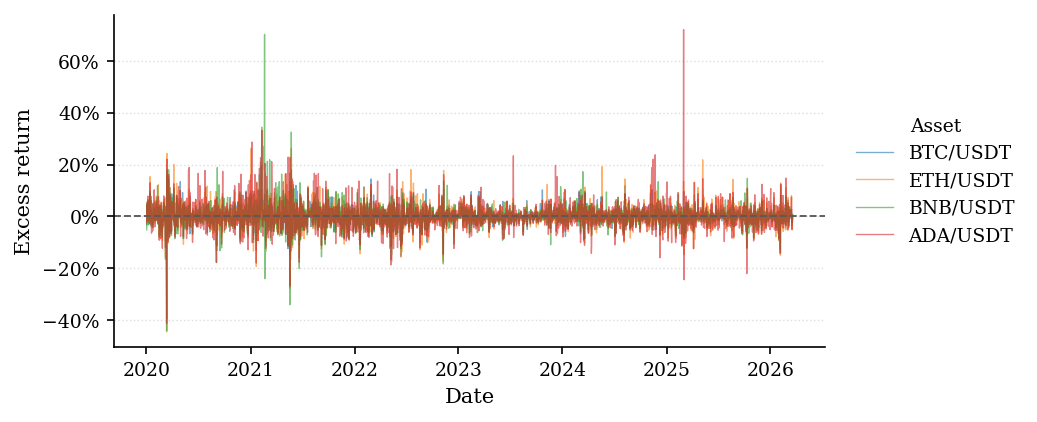
\includegraphics[width=0.95\textwidth]{figures/excess_returns.png}
    \caption{Daily excess return series for BTC/USDT, ETH/USDT, BNB/USDT, and ADA/USDT.}
    \label{fig:excess_returns}
\end{figure}

At daily frequency, the per-period risk-free rate is economically negligible relative to cryptocurrency price movements. For example, a 5\% annual rate is only about $0.014\%$ per day, compared with typical daily crypto volatility of 3\%--5\% or more. As a result, subtracting $\riskfree$ has almost no effect on returns, signals, or backtest results at this horizon.

\section{Strategy}

Both strategies are implemented using the same period for training and testing. The initial portfolio value is set at $V_0 = \$10{,}000$, subject to a firm gross exposure constraint of $\sum_i |\theta_{t,i}| \leq \$100{,}000$.

\subsection{Strategy 1: Trend-Following}

\subsubsection{Rationale}

As outlined in \citep{liu_tsyvinski_2021}, cryptocurrency assets, similarly to other asset classes exhibit time series momentum behaviour. The intuition being that assets which have had positive excess returns tend to sustain that trend for some time in bull markets, the opposite is also observed with negative excess returns during bear markets.

\subsubsection{Signal Construction}
For each asset $i$ at time $t$, I compute a volatility-normalised trend signal. This is done in two stages. First, I compute the raw trend $\tau^{\mathrm{raw}}_{i,t}$, which captures the deviation of the close price $p_{i,t}$ from its $w$-bar moving average:

\begin{equation}
    \tau^{\mathrm{raw}}_{i,t} = \frac{p_{i,t}}{\mathrm{MA}_{i,t}(w)} - 1.
\end{equation}

where $\mathrm{MA}_{i,t}(w)=\frac{1}{w}\sum_{k=0}^{w-1} p_{i,t-k}$.
I standardise this signal by dividing it by the rolling standard deviation of simple returns over a $w_{\mathrm{vol}}$-bar window:

\begin{equation}
    z_{i,t} = \frac{\tau^{\mathrm{raw}}_{i,t}}{\sigma_{i,t}(w_{\mathrm{vol}})}.
\end{equation}

The z-score is clipped and the position direction is determined by a threshold with a dead zone to prevent noisy oscillations from needlessly increasing costs.

\subsubsection{Position Sizing using Mean Variance Optimisation}

For position sizing I implement MVO using shrinkage estimation of the rolling covariance matrix \citep{ledoit2004} with cvxpy quadratic programming.

On bars where the signal is active ($\lvert z_{i,t} \rvert > \delta$), the raw weight is $w^{\mathrm{raw}}_{i,t} = \tau^{\mathrm{raw}}_{i,t}$, whereas for inactive bars it is zero.

The optimisation step solves
\[
\max_w \; \mu^\top w - \frac{\gamma}{2} w^\top \hat{\Sigma}_t w
\quad \text{subject to} \quad \|w\|_1 \leq 1,
\]
with $\gamma = 1$, where $\mu$ is proxied by the volatility scaled signal and $\hat{\Sigma}_t$ is the Ledoit Wolf shrinkage covariance estimate. While a diagonal inverse volatility approximation performed better in sample, the full MVO specification was preferred because it captures cross-asset covariance and should be more robust when correlations spike in stressed markets. Positions are rebalanced every $n$ days, a configurable frequency.

\subsubsection{Parameter Selection}

The parameters for the strategy were selected using a walk forward validation procedure. An untouched test window of 126 consecutive daily observations (about 4.1 calendar months in a market that trades seven days per week) was kept for out of sample testing. This process used folds of 600 bars and a validation window of 100 bars, advancing by 100 bars per fold. This yielded 15 walk-forward folds of which every second were evaluated.

The search grid used the following parameters: moving-average window $w$, volatility window $w_{\mathrm{vol}}$, dead-zone threshold $\delta$, rebalancing frequency $n$, and gross utilisation $u$. The signal clip was fixed at $\pm 5$, and the gross cap at $\$100{,}000$.

Each candidate combination is evaluated across all folds and the sharpe ratio is computed. The combinations are then selected based on a stability penalised mean validation Sharpe:

\begin{equation}
    \mathrm{score} = \bar{S}_{\mathrm{val}} - \lambda\,\mathrm{std}(S_{\mathrm{val}}).
\end{equation}

where $\bar{S}_{\mathrm{val}}$ is the mean Sharpe ratio across folds, and $\mathrm{std}(S_{\mathrm{val}})$ is the cross-fold standard deviation. I set $\lambda = 0.1$ as the stability penalty. A candidate must have a positive mean Sharpe, and at least $55\%$ of folds must exhibit positive Sharpe ratios.

This procedure selects $w = 140$ days, $w_{\mathrm{vol}} = 30$ days, $\delta = 1.0$, $n = 10$ days, and $u = 0.10$. This combination yields a mean Sharpe of $0.464$, with $62.5\%$ positive folds as well as an adjusted score of 0.306. This long moving average window is consistent with the findings of \citep{moskowitz2012timeseriesmomentum}.

\subsection{Strategy 2: BTC Dominance Mean-Reversion}

\subsubsection{Rationale}

Bitcoin is the largest asset among cryptocurrencies, making up the majority of the market cap of the cryptocurrency market \citep{coinmarketcap2026}. The signal in this strategy sets BTC dominance as BTC's share of aggregate notional trading volume across cryptocurrencies. During regimes of fear and uncertainty this dominance tends to spike as crypto investors de risk into the most liquid crypto asset. The mean reversion strategy buys a basket of altcoins, anticipating a rotation back into these assets as the regime shifts.

\subsubsection{Signal Construction}

The signal is built from a notional dominance ratio $D_t = \frac{\mathrm{notional}^{\mathrm{BTC}}_t}{\sum_j \mathrm{notional}^{j}_t}$. The notional is defined as close price times volume for each asset.

The first indicator for the strategy is a 20 day z-score of the dominance level:

\begin{equation}
    z_t^{\mathrm{dom}} = \frac{D_t - \bar{D}_t^{(20)}}{\hat{\sigma}_{D,t}^{(20)}}.
\end{equation}

The second indicator is a 3 day rate of change of dominance $ROC_t=D_t-D_{t-3}$ which serves as a way to prevent the strategy getting caught in long-term market shifts.

Entry to the strategy happens when both of these metrics exceed their 80th and 95th 126 day rolling percentile respectively. The position exits when the dominance score drops to zero or a holding period of 7 days passes. I did experiment with a crash filter however the Optuna search consistently favoured the no filter configuration.

\subsubsection{Parameter Selection}

The signal parameters were tuned using Bayesian hyperparameter optimisation using Optuna's Tree structured Parzen Estimator (TPE) sampler with 80 trials. The search space covers: entry percentile, exit z-score, maximum holding period, ROC percentile, crash threshold and gross utilisation.

The walk forward scoring function is:

\begin{equation}
  score = \bar{S}_{val} - 0.15\cdot std(S_{val})-P_{inactivity}
\end{equation}




% =============================================================================
% SECTION 3 — Transaction Costs [10 points]
% =============================================================================
\section{Transaction Costs}

For transaction costs, I use the Abdi--Ranaldo close--high--low spread estimator \citep{AbdiRanaldo2017}. It estimates a proportional effective spread when quote data are unavailable. With $m_t=(\ln h_t+\ln l_t)/2$ denoting the log mid-range, the two-day squared-spread observation is

\begin{equation}
  \hat{s}_t^{2} = 4\left(\ln c_t-m_t\right)\left(\ln c_t-m_{t+1}\right).
\end{equation}

Abdi and Ranaldo define two corrections for negative sample moments. The monthly-corrected estimator is $\sqrt{\max\{N^{-1}\sum_t \hat{s}_t^2,0\}}$; the two-day-corrected estimator is $N^{-1}\sum_t\sqrt{\max\{\hat{s}_t^2,0\}}$. The backtest uses a 21-day window, divides the full spread by two, and lags that half-spread by one completed bar before charging traded notional.

A code audit found that the earlier implementation instead applied an absolute value to a negative 21-day mean. This is neither correction defined in the paper and converts wrong-signed estimation noise into a positive cost. The implementation now supports only the two published corrections. The monthly-corrected version is the primary restatement for the frozen strategies, and the two-day-corrected version is reported as a sensitivity case. No signal, parameter, trade, position, or turnover series was retuned.

\subsection{Cost Sensitivity}

For the fixed relative-value candidate discussed below, the monthly correction implies a turnover-weighted one-way execution cost of 14.9 basis points, while the two-day correction implies 42.3 basis points. The observed break-even is 35.0 basis points. The correction choice therefore changes the sign of the net result and must be shown rather than hidden behind one ``conservative'' label. Fixed 5, 10, 20, and 40 basis-point scenarios provide transparent reference points.


\begin{figure}[htbp]
    \centering
    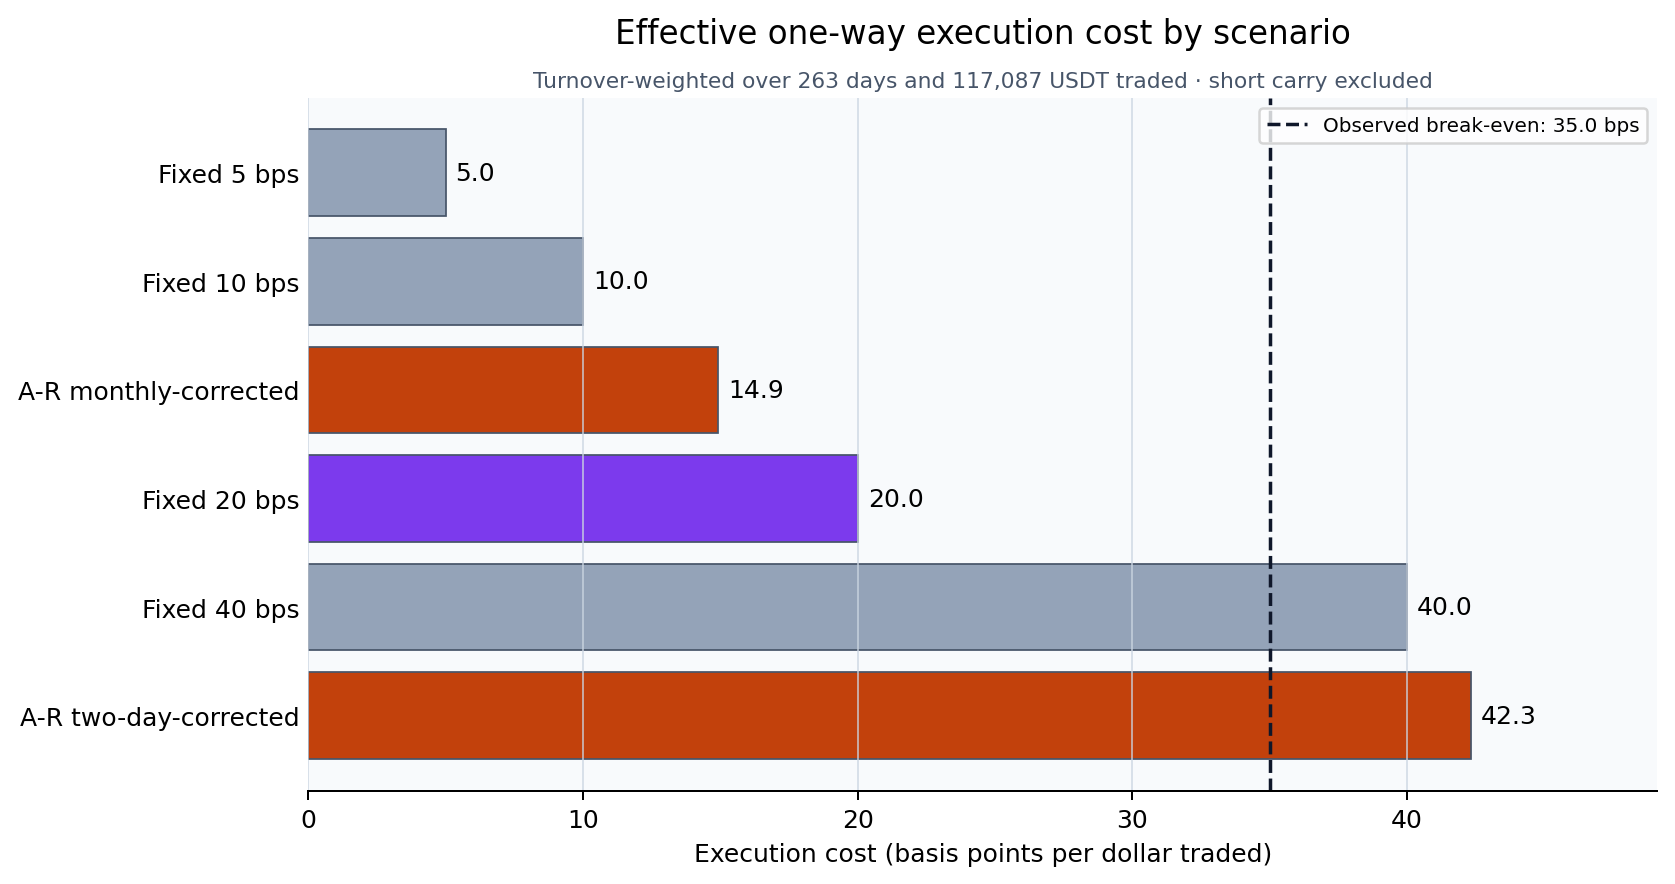
\includegraphics[width=0.92\textwidth]{figures/strategy2_candidate_effective_cost.png}
    \caption{Turnover-weighted one-way execution costs for the unchanged relative-value candidate. Short carry is excluded from the basis-point comparison and included in every net result.}
    \label{fig:costs}
\end{figure}




\section{Performance}

Strategy 1 keeps total exposure fixed at \$10,000 throughout the backtest, regardless of portfolio gains or losses. This maintains stable daily dollar risk, although effective leverage relative to portfolio value changes over time. This means that the maximum one-day profit or loss is bounded by fixed exposure multiplied by the largest absolute asset return on that day.

Strategy 2 is designed to trade at a target exposure of \$20,000. In normal conditions, that is the amount the strategy puts to work. The \$100,000 gross exposure limit is a set constraint, while the $10 \times V_t$ term acts as a safety check so the strategy never takes on more than 10 times its current equity. In practice, this means the strategy usually trades with a fixed \$20,000 exposure, but if the portfolio value falls far enough, the position size is automatically reduced to avoid excessive leverage.

\clearpage
\subsection{Metrics}

\begin{table}[htbp]
\centering
\small
\setlength{\tabcolsep}{4pt}
\renewcommand{\arraystretch}{0.95}
\begin{tabular}{lcccc}
\toprule
& \multicolumn{2}{c}{Strategy 1} & \multicolumn{2}{c}{Strategy 2} \\
\cmidrule(lr){2-3} \cmidrule(lr){4-5}
Metric & IS & OOS & IS & OOS \\
\midrule
Sharpe Ratio              & 0.923  & 1.300  & 0.343  & -2.912 \\
Sortino Ratio             & 1.151  & 1.838  & 0.197  & -1.377 \\
Calmar Ratio              & 0.825  & 3.324  & 0.105  & -1.927 \\
Ann. Return (\%)          & 18.38  & 12.56  & 6.30   & -14.0  \\
Max Drawdown (\%)         & -22.3  & -3.8   & -59.9  & -7.3   \\
Total Net PnL (\$)        & +31,903 & +2,431 & +6,818 & -1,222 \\
Gross PnL (\$)            & +42,332 & +2,511 & +30,866 & -596 \\
Total Turnover (\$)       & 1,253,508 & 13,503 & 2,260,369 & 80,079 \\
Return on $V_0$ (\%)      & 319.0  & 24.3   & 68.2   & -12.2  \\
Active Days (\%)          & 93.5   & 100.0  & 9.0    & 2.4    \\
Avg.\ Holding Period (days) & 10 & 10 & 3.6 & 1.5 \\
\bottomrule
\end{tabular}
\caption{Original submitted performance metrics for both strategies (net of the estimator implementation used at submission). These historical rows are retained for provenance; the paper-correct cost restatement is reported separately below. Ratios use the project's 252-observation annualisation convention. Strategy 1 holdout start equity: \$41{,}903. Strategy 2 is tuned with $u = 2.0$ (\$20{,}000 gross).}
\label{tab:strategy_performance_combined}
\end{table}
\FloatBarrier

The submitted table records the model-selection outcome and the claims made at submission, but its net figures should not be interpreted as paper-correct Abdi--Ranaldo estimates after the audit above. Its still-valid qualitative points are that Strategy 1 was highly concentrated in BTC during the holdout and Strategy 2 was episodic, leveraged, and supported by very few trades. Current cost-dependent interpretation relies on the restated frozen evaluation below.

The original holdout strengthens the case for Strategy 1. It records a Sharpe ratio of 1.30 with a shallow maximum drawdown of only $-3.8\%$, while BTC buy-and-hold over the same window returns $-26.2\%$ with a Sharpe of $-1.16$. The exposure breakdown shows that BTC accounted for the vast majority of gross exposure during this period. Strategy 2 instead lost money as the expected altcoin rebound did not materialise. Its two qualifying holdout trades are too few for a precise performance estimate, but the negative economic result is retained without retuning.

\subsection{Continuous Post-Selection Evidence}

Both frozen specifications were subsequently run through 4 August 2026. Covering the dates of the original 126-observation holdout and 137 completed post-freeze daily observations gives one uninterrupted 263-observation period from 15 November 2025. The metrics are recomputed from one stateful run of the hashed frozen evidence pipeline using the monthly-corrected spread estimate, not by adding rounded values from the submitted table. This is a cost-method restatement with unchanged parameters and trades. The longer window does not replace the original holdout: because its first segment was already observed when the strategies were frozen, it is explicitly treated as post-selection evidence.

\begin{table}[htbp]
\centering
\small
\setlength{\tabcolsep}{7pt}
\renewcommand{\arraystretch}{0.95}
\begin{tabular}{lrr}
\toprule
Metric & Strategy 1 & Strategy 2 \\
\midrule
Net Return (\%)          & +9.54 & -6.96 \\
Annualised Return (\%)   & +9.13  & -6.68 \\
Sharpe Ratio              & 1.251  & -1.521 \\
Maximum Drawdown (\%)    & -4.30  & -6.96 \\
Gross PnL (\$)            & +4,563 & -1,365 \\
Transaction Costs (\$)    & -98   & -540 \\
Net PnL (\$)              & +4,465 & -1,905 \\
Total Turnover (\$)       & 90,823 & 282,099 \\
Mean Gross Exposure (\$)  & 9,953  & 1,065 \\
Activity                   & 100.0\% of days & 7 entries / 14 days \\
Entry-Count Evidence Gate  & -- & 7 / 20 minimum; 30 preferred \\
\bottomrule
\end{tabular}
\caption{Continuous post-selection results from 15 November 2025 to 4 August 2026, net of monthly-corrected Abdi--Ranaldo costs. Annualised figures use 252 observations per year for comparability with the submitted analysis.}
\label{tab:post_selection_performance}
\end{table}
\FloatBarrier

Strategy 1 returned $9.54\%$ with a Sharpe ratio of 1.251 and a $-4.30\%$ maximum drawdown, while BTC buy-and-hold and the equal-weight four-asset basket returned $-32.23\%$ and $-42.29\%$, respectively. The result remains concentrated: mean absolute BTC exposure was \$7,718 of \$9,953 mean gross exposure. Strategy 2 returned $-6.96\%$ and lost \$1,365 before \$540 of estimated costs. Its mean exposure across all observations is low because it was active for only 14 days; when active, gross exposure remained approximately \$20,000.

Because Strategy 2 is episodic, elapsed days cannot substitute for trade events. A rule registered on 5 August 2026, after seven entries were observed, sets 20 as the bare minimum and 30 as preferred. Return and Sharpe are therefore descriptive, not reliable inference. At seven entries per 263 days, linear planning extrapolation implies roughly 751 total days, or 488 more; this is not a forecast or guarantee.

\subsection{Post-Hoc Strategy 2 Research Lead}

The frozen failure above remains the canonical Strategy 2 result. A separate adaptive retrospective programme retained all negative paths while screening 24 candidate variants across entry confirmation, liquid baskets, fixed holding periods, and relative-value constructions. Entry confirmation produced excessive turnover; smaller baskets and fixed long-only holds remained gross-negative. The first economically different lead was a $1\times$ gross, seven-day trade allocating 50\% long to an equal-weight ETH/BNB/SOL basket and 50\% short to BTC after the unchanged entry signal.

This candidate earned \$465 gross over the same 263-day period. With a fixed 20 basis-point charge per dollar traded plus a 10\% annual BTC-short carry stress, it returned $+1.54\%$ (\$176 net), with a descriptive Sharpe of 0.43 and a $-2.09\%$ maximum drawdown. The paper's monthly-corrected Abdi--Ranaldo estimator returned $+2.67\%$ (\$235 net; 14.9 basis points one way), whereas its two-day-corrected estimator returned $-1.38\%$ (-\$86 net; 42.3 basis points). Fixed 5, 10, 20, and 40 basis-point scenarios are all retained; the 40 basis-point case lost \$59. The observed break-even was approximately 35 basis points one way.

\begin{figure}[htbp]
    \centering
    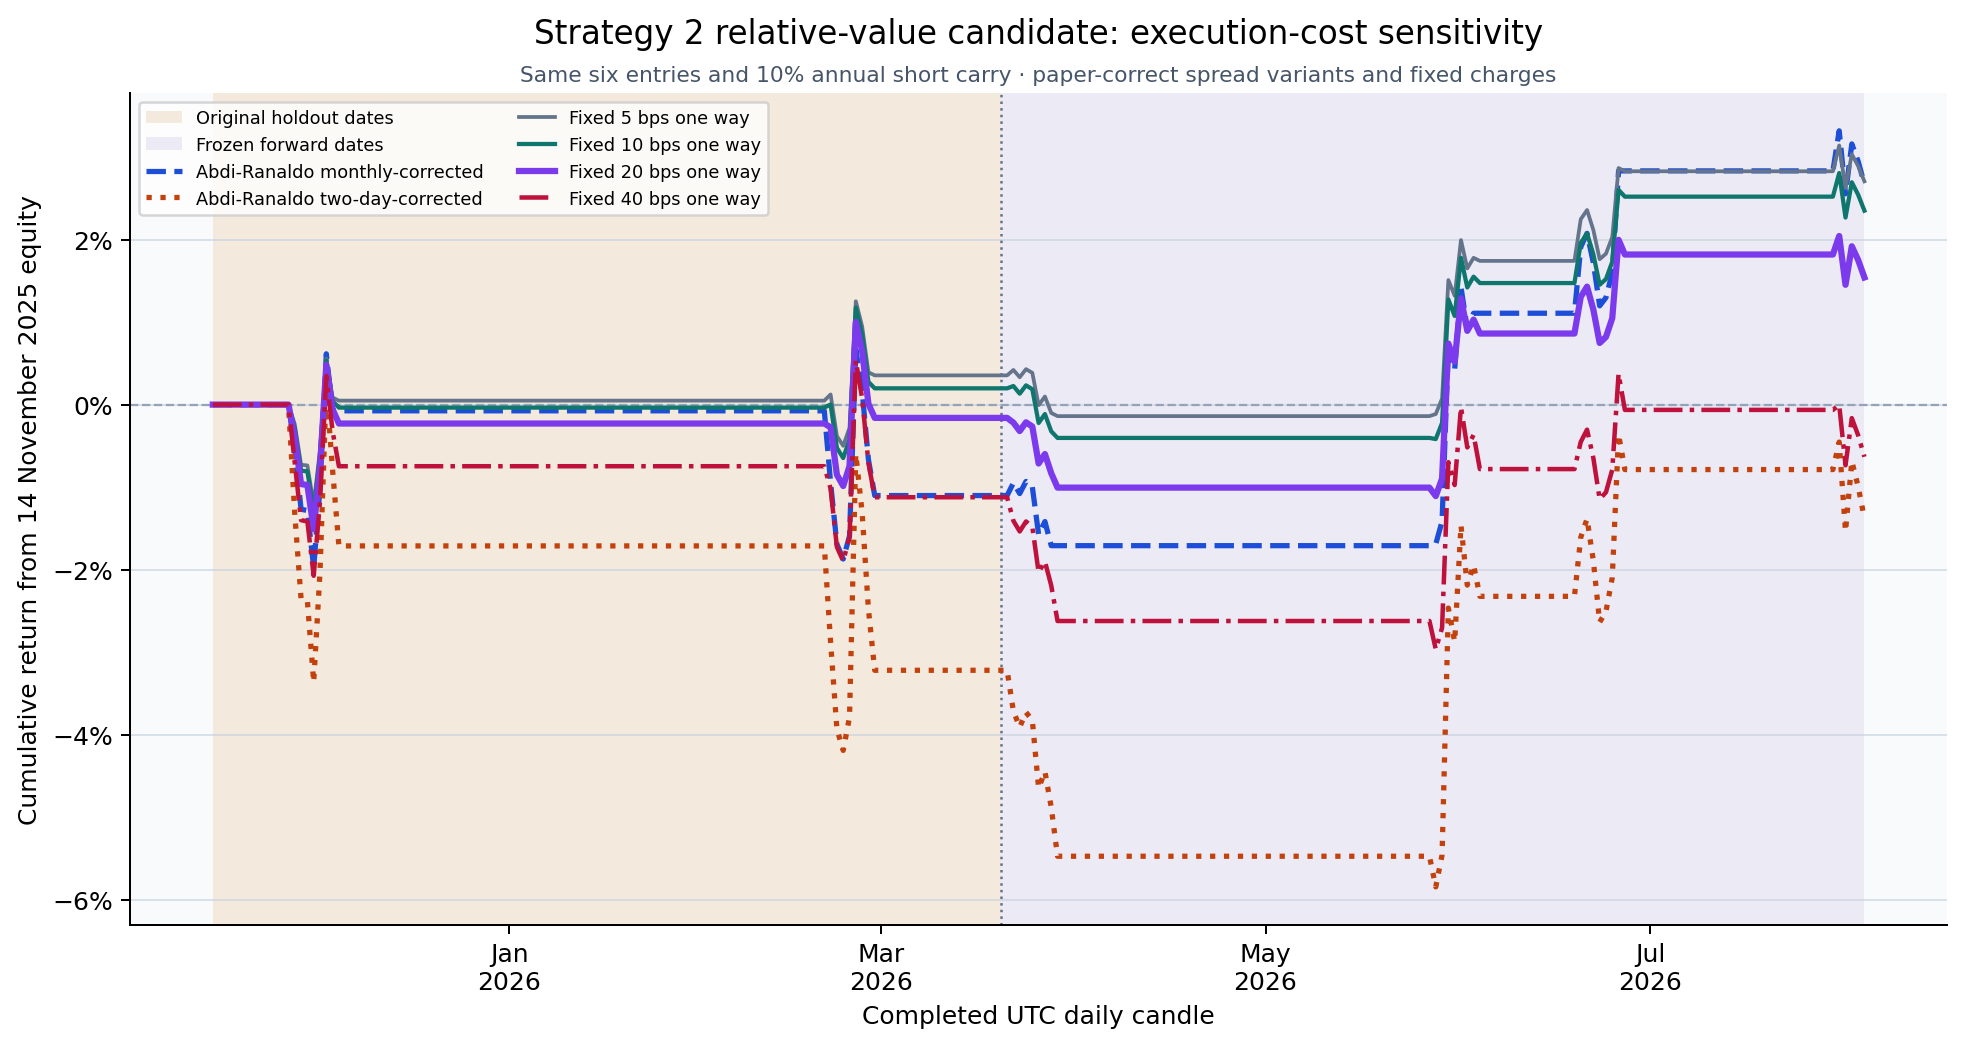
\includegraphics[width=0.92\textwidth]{figures/strategy2_candidate_cost_sensitivity.png}
    \caption{Cumulative return of the unchanged six-entry Strategy 2 candidate under both paper-corrected spread estimators and all four fixed one-way execution-cost scenarios.}
    \label{fig:strategy2_candidate_costs}
\end{figure}

The evidence is insufficient for a performance claim. Only six entries occurred; the original holdout segment was negative; the largest winner exceeded total net profit; and a seeded seven-day moving-block bootstrap gave a 95\% return interval of $[-3.34\%,+7.51\%]$. The search was adaptive and subject to look-elsewhere and forking-path effects. I therefore describe it only as a cost-conditional research lead. Its specification is fixed for future monitoring and requires 20 new entries from 5 August 2026 onward (30 preferred), including realised execution and funding costs, before interpretation is reconsidered.


\begin{figure}[htbp]
    \centering
    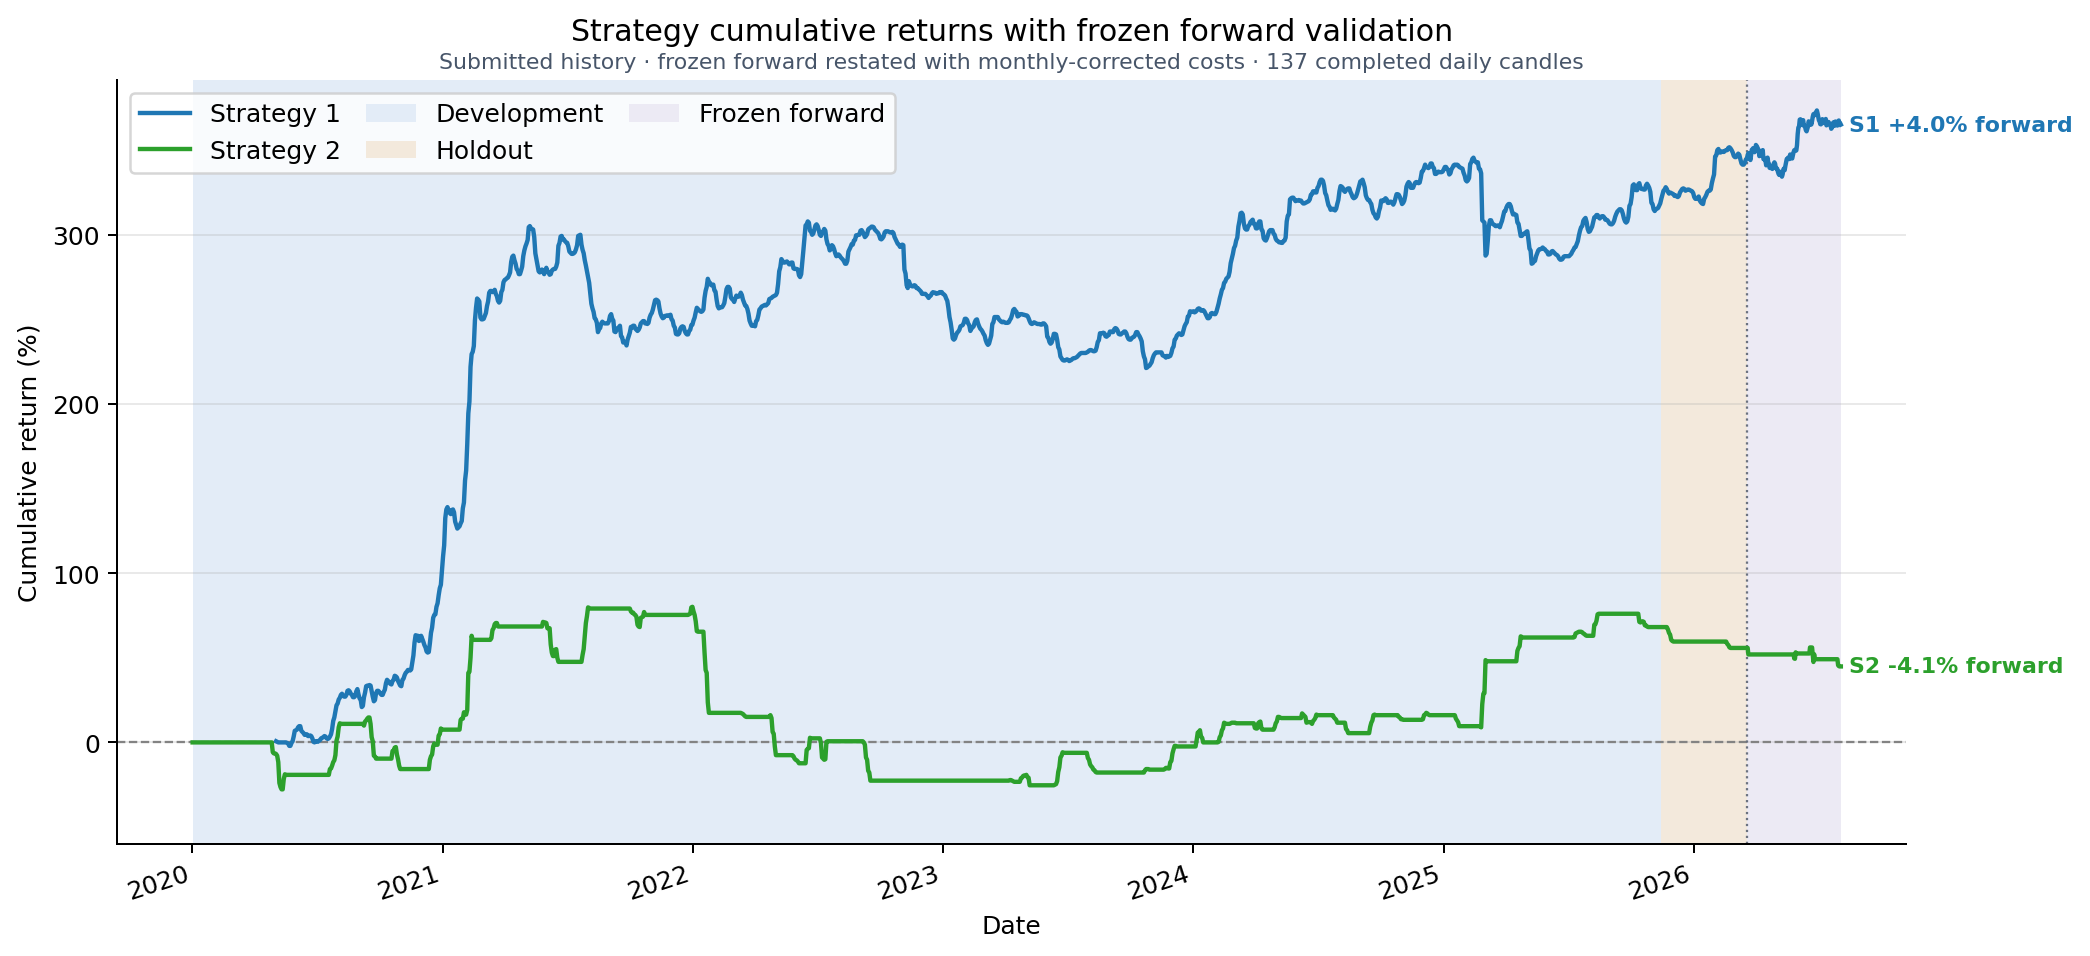
\includegraphics[width=0.85\textwidth]{figures/readme_performance_overview.png}
    \caption{Submitted historical cumulative-return paths extended with monthly-corrected accounting for 137 post-freeze observations. Shading separates development, original holdout, and frozen-forward evidence.}
    \label{fig:returns}
\end{figure}

\FloatBarrier
\thispagestyle{fancy}

\section{Next Steps}
Both strategies remain regime dependent. Strategy 1's positive result is heavily concentrated in BTC, so a pre-specified expansion of the asset universe could improve diversification. The 263-observation post-selection period improves on the original short holdout but covers only about 8.6 calendar months, while frozen Strategy 2 generated just seven of the 20 entries required by its bare interpretive gate and remained negative even after the cost correction. Frozen monitoring should continue unchanged. The separate relative-value lead should likewise remain fixed and accumulate its own 20 new entries, with realised execution and funding records, rather than be promoted from its retrospective and cost-conditional result. Because the two published Abdi--Ranaldo corrections bracket the observed break-even, realised quotes, fees, slippage, and funding are more decision-relevant than choosing the favourable estimator. Any further regime filter or capital-allocation framework must be registered as another experiment and added to the complete search ledger.

\nocite{*}
\bibliographystyle{plainnat}
\bibliography{references}

\end{document}
